\documentclass[a4paper,10pt]{llncs}
\usepackage[utf8]{inputenc}
\usepackage[margin=0.8in]{geometry}

% Packages for protocol graph.
\usepackage{amsmath}
\usepackage{tikz}

%opening
\title{Petrol rationing smartcard project}
\subtitle{Design document - Group 5 (TU/e)}
\author{Alvin Cai - s4404114 \\ Romanos Dodopoulos - s4415191 \\ Alexandru Geana - s4420438 \\ Saurabh Kulkarni}
\institute{}

\begin{document}

\maketitle

\section{Introduction}
\subsection{Purpose of this document}

Since the war "somewhere in the Middle East", the amount of petrol available to the general population has drastically decreased. As a result, the government has decided to implement a nation wide rationing system to ensure that all citizens have equal access to the resource. This document is meant to describe the involved parties, system requirements and design, reasoning and decisions and finally the implementation details together with the challenges that were faced.

\subsection{Target audience}

This document is targeted towards government officials who are charged with seeing this project to completion, implementors of the rationing system as well as any stakeholders interested in specific details of the design process and underlying decisions. The sections which describe the requirements and the protocol specifications are meant for the hardware manufacturers. The petrol companies and gas station managers may also find this document informative and useful when trying to understand the finer details of the system. Lastly, the document should be made public such that card owners can access it for the purpose of understanding how the system deals with lost cards.

\subsection{Structure}

The document is structured into seven sections as follows:
\begin{enumerate}
  \item The introduction.
  \item Use cases for the petrol rationing system.
  \item A listing of all the assets which make up the system.
  \item A listing of all parties involved in this project and their responsibilities.
  \item The model of the attacker which we considered when designing the protocol.
  \item The security requirements which the protocol implements to mitigate any possible attacks.
  \item The full design description which includes the security rationale.
\end{enumerate}

\section{Use Case}
The ration card is personalised in the backend before it is issued to the user. Users charge their ration cards at charging terminals to increase the petrol balance. Petrol pumps are equipped with card terminals and they only supply petrol upon presentation of a valid ration card with sufficient balance.

\subsection{Card Personalisation and Issue}
\label{personalisation}
\begin{enumerate}
  \item Car owners apply to the government for personalised ration cards.
  \item The government verifies that the applicant does not currently have an active card and generates a personalised card loaded with:
	\begin{itemize}
	  \item Two PKI certificates, one each for key exchange and digital signature, signed by the Intermediate Cards Certificate Authority (CA).
	  \item The corresponding private keys
	  \item Intermediate Pump CA and Intermediate Charging CA
	  \item Randomly generated secret PIN.
	\end{itemize}
  \item The smartcard and secret PIN are delivered to the car owner through a secure physical channel.
  \item Disabled cards can be brought to personalisation centers to be unlocked.
\end{enumerate}

\subsection{Petrol Withdrawal and Card Charging}
\subsubsection{Authentication Phase}
Petrol terminals and charging terminals also contain two PKI certificates, one each for key exchange and digital signatures, signed by an Intermediate CA. Each terminal also stores its private key and the Intermediate Card CA. These certificates are used by the smartcard and terminal to mutually authenticate each other and establish an encrypted and authenticated connection. Thereafter, the card owner enters his secret PIN into the terminal. A maximum of three consecutive wrong attempts are allowed before the card is disabled. If the PIN is correct, then the user can proceed with filling petrol or charging the card, depending on the terminal.

\subsubsection{Petrol Filling Phase}
\begin{enumerate}
  \item The card sends to the pump terminal its current balance.
  \item The card owner inputs the amount of petrol he would like to fill into the vehicle and the terminal verifies that he has available balance.
  \item The pump then atomically reduces the balance on the card accordingly.
  \item The fuel is released.
  \item If the tank could not fit all the prepaid fuel, the terminal updates the balance on the card again.
  \item Signed logs are stored on the card to reflect the transaction.
  \item The card can be released.
\end{enumerate}

\subsubsection{Charging Phase}
\begin{enumerate}
  \item Charging terminals are connected to a backend database which maintains records of each card owner and their available petrol ration.
  \item Immediately after the mutual authentication, the charging terminal grabs the logs of the smartcard to clear the memory. In addition, the terminal safely stores the evidence of the performed transaction (logs) to the database in order to ensure non-repudiation.
  \item If the card has not been charged already on that month, the charging terminal increases the petrol ration in the card by the fixed monthly allowance ( 200 litres ) and updates the backend database. The allowance for the current month is added on top of the existing balance on the card, to the possible maximum value of a 2-byte unsigned value.
  \item If a card owner did not charge the card for the previous month, it does not carry over to the current month, but is forfeit.
\end{enumerate}


\subsubsection{Decommissioned Card}

\begin{enumerate}
  \item Cards may be decommissioned when they are lost or expire.
  \item Lost cards are reported to the government agency.
  \item The status of these cards is updated as revoked in the government database.
  \item Charging terminals no longer accept revoked cards and will disable them permanently.
\end{enumerate}


\section{Assets}

In order for the implemented system to work properly, a number of items are required. These items, both physical and non-physical, are listen below.

\begin{enumerate}
  \item Petroleum and fairness of its distribution.
  \item Integrity of petrol ration management and it's allocation to each car owner.
  \item Petrol and charging terminal stations.
  \item Smartcards for each car owner.
  \item Private keys of root and intermediate CAs.
  \item Private keys of smartcards and terminals.
  \item Symmetric Keys used for confidentiality and authentication of card-terminal communication.
  \item Smartcard PINs and appropriate management.
\end{enumerate}

\section{Stakeholders}
The implementation of a nation-wide petrol rationing system involves multiple parties. This section describes all engaged bodies and clearly states what aspects of the project are of concern to each of the stakeholders.

\subsection{Government}

The government can be considered one of the two main stakeholders in this project. They are the ones who initiated the project and who will manage it throughout its lifespan.

The main task of the government is to run the certificate authority system which is used to properly authenticate cards and terminals. They are responsible to keep the private keys secret. Moreover, they will generate-and-sign or revoke certificates for new or invalid hardware accordingly.

The end result of this project will help the government with distribution aspect of petrol on a nation-wide scale.

\subsection{Petrol Companies}

Petrol companies are responsible for issuing fuel to card owners upon presentation of legitimate cards. Petrol stations are required to issue the correct amount of fuel according to the value that is subtracted from the balance. The actual verification of the cards as well as the proper functioning of the terminals is not of concern to the petrol companies, but to the dedicated hardware.

\subsection{Car Owners}

Car owners form the last set of stakeholders that will make use of this system. Each card owner will obtain his monthly allocated fuel allowance. They are required to keep their cards safe and the PIN secret. In case the card is lost, then a fee is subtracted from the total balance stored in the backend, as described in Section \ref{subsection:nonrepud}.

\subsection{Hardware manufacturers}

Manufacturers deal with creating the hardware and software required to run the system. They are responsible for properly implementing the protocols in software.

\section{Attacker Model}
We define the opponent of the petrol rationing system based on his abilities and resources. Furthermore, we take into consideration the possible reasons why an opponent might want to attack the system. We take these assumptions into consideration when designing the security requirements for the system.

Assumptions regarding the capabilities of an opponent:
\begin{enumerate}
	\item The attacker is unable to solve the Elliptic Curve Discrete Logarithm Problem for curves over prime fields of sizes more than 193 bits.
	\item The attacker is unable to break AES encryption with key sizes of more than 128 bits.
	\item The attacker is unable to find meaningful collisions for digest of the SHA1 hashing algorithm.
\end{enumerate}

Assumptions regarding the end goals of an opponent:
\begin{enumerate}
	\item The opponent might try to obtain more petrol than the allowed monthly ration.
	\item The opponent may try to decrease the available balance of another person, without the victim getting his fuel.
	\item A denial of service attack may be desired in order to prevent other car owners from obtaining their legitimate fuel.
	\item Card owners may try to remove the card in the middle of the transaction in the hopes that fuel may be given without subtracting the fee from the available balance.
	\item People may try to steal the cards of other car owners in order to use the victim's monthly ration.
	\item Card owners with a low balance may declare their cards as stolen and request a new card with more credits than they have.
	\item Opponents may try to place skimming devices and attempt to clone cards in order to steal the monthly ration of the victims.
	\item Opponents with a good knowledge of the protocol details may try to create invalid smartcards and impersonate other people or create malicious terminals which replay transactions, steal PINs, do man-in-the-middle attacks or modify data in transit.
	\item The opponent may try to compromise private keys within petrol terminals so as to make fraudulent deductions and create public mistrust in the rationing system.
\end{enumerate}

\section{Security Requirements}
In order for the system to remain secure against possible attacks, a set of requirements is given. These requirements need to be met throughout the duration of the petrol rationing project. We prioritize the requirements into four categories according to the MoSCoW technique.

The system {\bf must} ensure that the following requirements are met:
\begin{enumerate}
  \item The private keys of the root certificate need to remain confidential at all times. Only the appropriate staff (appointed by the government) may have access to it.
  \item The private keys of the three intermediate certificates need to remain secret and only parties which are responsible for issuing new device certificates may have access to it.
  \item The private keys of the cards and terminals may not be made public and should only be stored on the devices themselves.
  \item Each card requires a PIN code which needs to remain secret. Only the owner of the card may know this code. The PIN is used to authenticate the owner to the card during operation.
  \item The protocol requires that the card and terminals be authenticated to each other. Integrity of the messages and freshness of the shared secrets between protocol executions also need to be ensured.
  \item The integrity of the balance value stored on the card needs to be assured. Changes to the balance, when topping up at charging terminals or subtracting at pump terminals, need to be logged accordingly. The system needs to be support non-repudiation of transactions which modify the balance.
  \item The charging terminals should always be connected to the backend (for instance, via internet or a private network) so that the logs are transferred from the card as described in Section (\ref{subsection:chargingterminal}).
  \item The availability of the petrol pumping terminals should be guaranteed even in the event of network loss.

\end{enumerate}

The system {\bf should} ensure that the following requirements are met:
\begin{enumerate}
  \item A certificate revocation list (CRL) or similar should be implemented such that terminals connected to the backend will be able to verify if a card has been invalidated.
\end{enumerate}

The system {\bf could} ensure the following features:
\begin{enumerate}
  \item Secret keys on cards could be automatically renewed at certain periods of time (for example, every year) when topping up the balance at charging terminals.
  \item The software running on the pump terminals could be implemented such that, if a connection to the backend is available, the logs are transferred from the card.
  \item It could be made possible for individual card owners to change their PINs.
  \item A limited CRL could be implemented for cards to have a limited list of terminals which have been revoked.
\end{enumerate}

The system {\bf will not} ensure any of the following:
\begin{enumerate}
  \item In case a card is lost, the exact balance available on the card will not be available any more. As such, a fee equal to the maximum petrol filling amount will be deducted as described in Section \ref{subsection:nonrepud}.
  \item The system will not offer any protection against inside attackers who have access to the private keys of certificates and who attempt to use them in malicious ways.
  \item The system does not protect against attacks which bypass the security checks of the petrol pump terminal to directly access petrol.
  \item We cannot assure the confidentiality of card PIN from shoulder surfing or other visual peeking.
\end{enumerate}

Next to these requirements, we also make the following assumptions regarding the hardware of the system (cards and terminals):
\begin{enumerate}
  \item The hardware is tamper resistant: (1) we assume that confidentiality and integrity of the data on the smartcard is guaranteed as-is and (2) in-transit data cannot be observed or altered by side-channel or physical attacks.
\end{enumerate}

\section{Design}

\subsection{Card Personalisation}
\label{Design:Personalisation}
During the Initialisation phase at a secure government site, a Personalisation Terminal will load the certs, private keys and PIN as mentioned in Section \ref{personalisation} into the ration card. This process causes the ration card to permanently transit from the Personalisation State to an Issued State.

\subsection{Certificate hierarchy}
In order to provide a system for mutual authentication and the required framework for sharing secrets, we decided to make use of a PKI system. For this project a custom Certificate Authority (CA) is used, which generates new certificates using a hierarchical approach, based on three separate tiers. Each of the devices, cards and terminals alike, will possess its own unique certificate.

At the top of the hierarchy is the root certificate which establishes the 1$^{st}$ tier. The root certificate will be valid for 30 years since it is meant to be constant throughout the lifetime of the project. This certificate will conceptually represent the government and any subsequent certificates signed by the root certificate will be considered trusted by the government. This certificate will not be used directly by any of the devices, but instead will be stored offline in secure hardware.

Signed by the root certificate will be three intermediate certificates, one for each type of device: cards, charging pumps and petrol pumps. This will be the 2$^{nd}$ tier of our CA hierarchy. These three intermediate certificates will have a shorter lifetime of 10 years. They will be used to validate devices which can be trusted within the petrol rationing system. Additionally, it will be possible to detect what type of devices are taking part during a session. Thus, terminals will only communicate with cards and cards will be able to distinguish between the type of terminals easily. Only the public key of each intermediate certificate will be available on the devices. The public key will be needed to verify signatures and validate devices. The private key will remain secret and will only be available to the parties which are responsible for issuing new cards and terminals.

The third tier of the CA will consist of certificates which will belong to individual devices. These certificates will be valid for 3 years and signed by the appropriate intermediate certificate, depending on the type of the device. Devices without a valid certificate, signed by the appropriate intermediate certificate, will not be accepted within the system. They will be rejected during the handshake between cards and terminals. Both the public and private keys of each 3$^{rd}$ tier certificate will be present on the devices. By using this approach, devices will be able to establish shared secrets using the Diffie-Hellman key exchange algorithm.

\subsection{Mutual Authentication and Secure Channel}
\label{section:mutualauth}
As specified in the previous chapter, the mutual authentication and sharing of secrets will be done using CAs based on three tiers. Due to the fact that the JavaCard API does not have dedicated classes for the X.509 format, striping down the system to its core components and use those primitives directly is the only alternative. As a result, the card will only store private-public keys, expiry date, the unique serial number and the signatures of the intermediate CA over these information to certify their validity. No extra information which is stored in regular certificates (e.g. common name) will be available on the devices.

The initial data exchange between a card and a terminal (either of the two terminal types) is meant to authenticate the devices to one another and establish a secure communication channel. For this purpose, we attempted to simulate the functionality of the TLS protocol (specifically ECDH-ECDSA).

The steps of this initial handshake are as follows:
\begin{enumerate}
 \item The terminal sends to the card an initial TERMINAL-HELLO message which includes a random nonce.
 \item The card receives the TERMINAL-HELLO message and sends back a CARD-HELLO message which includes a different nonce.
 \item The terminal sends to the card its public key and a signature of it and informs the card what type of terminal it is. The signature is made using the private key of the responsible intermediate certificate depending on the type of the terminal. The terminal does not send a timestamp since the card cannot accurately hold time on its own.
 \item After receiving the data from the terminal, the card verifies the signature against the stored public keys and in this way also verifies the type of terminal it is communicating with. If the signature matches, then the card sends to the terminal its own public key, the stored timestamp when the card's keypair expires and a signature of the two items. The trust store of the card contains the two public keys of the intermediate certificates used for the terminals. The public key of the root certificate is not used for verification purposes. The reason for this is that (a) for the root certificate we use keys much bigger than what the card supports, and (b) also to reduce the processing time required for signature verification.
 \item The terminal receives the data and verifies it accordingly. If the verification is passed, the terminal sends a CHANGE-CIPHER-SPEC message to the card, indicating that from then onwards all transmitted data will be encrypted.
 \item The card receives this message and sends its own CHANGE-CIPHER-SPEC.
 \item The two devices compute the same shared secret using the Diffie-Hellman key exchange algorithm. We will not be using the ephemeral version of the algorithm, but instead will use the static public and private keys of the devices. Since the algorithm requires that both parties have the appropriate private keys, the mutual authentication is established when both devices compute the same shared secret. This is the authenticated Diffie-Hellman key exchange algorithm which guards against MITM attack.
 \item After the shared secret has been calculated, a pseudo-random function is used together with the two exchanged nonces and the shared secret to generate keys for encryption and message authentication codes. These nonces help to ensure that the keys used are fresh, thus preventing replay attacks.
\end{enumerate}

Once these steps have occurred, the two devices have the assurance about each other's identity and can communicate via a confidential and authenticated channel.

\subsection{Petrol Pumping Terminal}
\label{Design:PetrolPT}
After mutual authentication and PIN entry, the petrol pump and ration card follow the communication protocol described in Figure \ref{figure:petrol}, to securely deduct the card balance in exchange for fuel. Signatures are performed on the transaction and stored in the log file of the card for non-repudiation purpose.

All necessary information required for this protocol are stored locally in the petrol terminal and card. As such, there is no need for online access to the backend database thus avoiding the risk of network based DoS attacks. However, if OCSP is implemented as described in \ref{section:lost} then a network connection is required. In this case, a DoS attack prevents checking of the revocation status but not the core functionality.

\usetikzlibrary{matrix,shapes,arrows,positioning,chains, calc}

\begin{figure}[h!]

\begin{tikzpicture}
\matrix (m)[matrix of nodes, column  sep=1.2cm,row  sep=0.5mm, nodes={draw=none, anchor=center,text depth=0pt} ]{
Smart Card & & Pump terminal\\
Perform basic checks $($Sect \ref{section:lost}$)$ & & & $(1)$ \\
$B\leftarrow$Balance & & & $(2)$ \\[-1mm]
& Send $B$ & & $(3)$ \\[-1mm]
&  & Display $B$ & $(4)$ \\
&  & $A\leftarrow$Read amount & $(5)$ \\
&  & Verify $A\leq$$B$ & $(6)$ \\
&  & $m\leftarrow$
$\begin{cases}
Certificate ID_t\\
$B'=B-A$\\
Date\\
\end{cases}$ & $(7)$ \\[+4mm]
&  & $S_{t}\leftarrow\{|\#(m)|\}C_{t}$ & $(8)$ \\[-1mm]
\color{blue}&\color{blue} Send $m$,$S_{t}$ & & $(9)$ \\[-1mm]
\color{blue}Verify $B'<B$ & & & $(10)$ \\
\color{blue}$S_{c}\leftarrow\{|\#(m)|\}C_{c}$ &  & & $(11)$ \\
\color{blue}Store $\{m,S_{t},S_{c}$\} in log &  & & $(12)$ \\
\color{blue}Update log index &  & & $(13)$ \\[-1mm]
\color{blue}&\color{blue} Send ACK & & $(14)$ \\[-1mm]
&  & $F\leftarrow$Release fuel & $(15)$ \\
&  & If $F<A$, repeat steps 7-13, where $A=F$ & $(16)$ \\
&  &  & \\
};

% Header
\draw[shorten <=-1cm,shorten >=-1cm] (m-1-1.south east)--(m-1-1.south west);
\draw[shorten <=-1cm,shorten >=-1cm] (m-1-3.south east)--(m-1-3.south west);

% Arrows
\draw[shorten <=-1cm,shorten >=-1cm,-latex] (m-4-2.south west)--(m-4-2.south east);
\draw[shorten <=-1cm,shorten >=-1cm,-latex] (m-10-2.south east)--(m-10-2.south west);
\draw[shorten <=-1cm,shorten >=-1cm,-latex] (m-15-2.south west)--(m-15-2.south east);
\end{tikzpicture}
\\Note: Steps 9 to 14 (in Blue) are an atomic operation
\caption{\label{figure:petrol}Petrol Terminal and Smartcard Communication}
\end{figure}


\subsection{Petrol Charging Terminal}
\label{subsection:chargingterminal}
After mutual authentication and PIN entry, the charging terminal and ration card follow the communication protocol described in Figure \ref{figure:charging}. The charging terminal is also used to retrieve the logs thus freeing the memory of the smartcard for additional logs. The logs constitute the non-repudiation evidence for any smartcard or terminal. Immediately after transferring the logs, the terminal verifies that the card is valid and that the balance is correct. This validation check involves checking that the card and terminal signatures of all transactions are valid, that the balance strictly decreases as time progresses and that the constraints described in Section \ref{section:lost} (i.e. not more than 5 transactions totalling 250 litres) are fulfilled. If any of these checks fail, then the card is revoked by toggling it's REVOKE-flag, again described further in Section \ref{section:lost}.

Afterwards there are three different cases according to the result of the verification. An error means that the card must be revoked and the process ends. Otherwise, we distinct two cases for whether the card had already been charged that month.

\usetikzlibrary{matrix,shapes,arrows,positioning,chains, calc}

\begin{figure}[h!]

\begin{tikzpicture}
\matrix (m)[matrix of nodes, column  sep=1.2cm,row  sep=0.4mm, nodes={draw=none, anchor=center,text depth=0pt} ]{
Smart Card & & Charging terminal\\
Perform PIN check $($Sect \ref{section:lost}$)$ & & & $(1)$ \\
\color{blue}&\color{blue} Send $Logs$ & & $(2)$ \\[-1mm]
\color{blue}&  &\color{blue} Store $Logs$ & $(3)$ \\[-1mm]
\color{blue}&\color{blue} 'Clear $Logs$'  & & $(4)$ \\[-1mm]
\color{blue} Clear $Logs$ &  &  & $(5)$ \\
& & $B\leftarrow$Extract balance from $Logs$ & $(6)$ \\
& & Verify $B$ to DB & $(7)$ \\
\color{red}& &\color{red} If 'error': & $(8)$ \\[-1mm]
\color{red}&\color{red}REVOKE & & $(9)$ \\[-1mm]
& & If 'ok': release card & $(10)$ \\
& & If 'charge': $B'=B+200$ & $(11)$ \\[-1mm]
& & $m\leftarrow$
$\begin{cases}
Certificate ID_t\\
B'\\
Date\\
\end{cases}$ & $(12)$ \\[+1mm]
\color{blue}&\color{blue}Send $m$ & & $(13)$ \\[-1mm]
\color{blue}$S_{c}\leftarrow\{|\#(m)|\}C_{c}$ &  & & $(14)$ \\
\color{blue}Replace $B=B'$& & & $(15)$ \\[-1mm]
\color{blue}&\color{blue} Send $S_{c}$ & & $(16)$ \\[-1mm]
\color{blue}&  &\color{blue}$S_{t}\leftarrow\{|\#(m)|\}C_{t}$ & $(17)$ \\[-1mm]
\color{blue}&  &\color{blue}Store $m,S_{t},S_{c}$ in DB & $(18)$ \\[-1mm]
& & Finish & $(19)$ \\[-1mm]
};

% Header
\draw[shorten <=-1cm,shorten >=-1cm] (m-1-1.south east)--(m-1-1.south west);
\draw[shorten <=-1cm,shorten >=-1cm] (m-1-3.south east)--(m-1-3.south west);

% Arrows
\draw[shorten <=-1cm,shorten >=-1cm,-latex] (m-3-2.south west)--(m-3-2.south east);
\draw[shorten <=-1cm,shorten >=-1cm,-latex] (m-5-2.south east)--(m-5-2.south west);
\draw[shorten <=-1cm,shorten >=-1cm,-latex] (m-10-2.south east)--(m-10-2.south west);
\draw[shorten <=-1cm,shorten >=-1cm,-latex] (m-14-2.south east)--(m-14-2.south west);
\draw[shorten <=-1cm,shorten >=-1cm,-latex] (m-17-2.south west)--(m-17-2.south east);

\end{tikzpicture}
\\Note: Steps 2 to 5 as well as 13 to 18 (in Blue) are atomic operations.
\caption{\label{figure:charging}Charging Terminal and Smartcard Communication}
\end{figure}



\subsection{Non-repudiation}
\label{subsection:nonrepud}
To prevent card owners from disputing filling fuel and the collection of monthly petrol allowance, all transactions will be digitally signed by both the terminal and the card and, eventually, stored in the database. These can then be referenced in cases of disputes. As such, in addition to the certificates used in Section \ref{section:mutualauth} for mutual authentication, both cards and terminals have a second certificate used for digital signatures which adheres to the same certificate hierarchy.

Every transaction between a card and a petrol terminal is first stored in the card's logbook. This logbook has space for 6 logs. Each log includes a message (comprising of the certificate ID of the terminal, updated balance and the date of transaction) and signatures from both the petrol terminal and the card on this message.

When the card is plugged into a charging terminal, these logs are uploaded automatically into the backend database and safely stored. Whenever the charging terminal updates the card balance with its monthly allowance, a log entry will similarly be created.

Finally, card owners are responsible for not losing the card. In case that a card is missing or stolen the balance is reduced according to the defined maximum fuel filling amount (250 litres) per month. This is an inevitable consequence of keeping the petrol pumping phase off-line.

\subsection{Lost Cards and Compromised Terminals}
\label{section:lost}
\subsubsection{Lost Cards}
Cards may be misplaced or stolen. The first layer of defence against abuse by an attacker is the card PIN. This 4-digit PIN would have been randomly generated during card personalisation and not known to the attacker. PIN authentication is also carried out only after an authenticated and encrypted channel is created between the card and terminal - it cannot be eavesdropped by a MITM attack or a fake terminal.

Additionally, cards only allow three consecutive wrong PIN entries before the card is locked and all functionality prohibited. Locked cards can be re-activated by the legitimate card owner at government centres where human staff can physically authenticate the card owner e.g. against identity cards.

The next layer of defence is for the Government CA to revoke cards which are reported to be misplaced or stolen. This is updated in the backend database to which charging terminals are connected. When a revoked card is presented to a charging terminal, the charging terminal will disable the card by toggling a 'REVOKE-FLAG' within the card.

A third layer of defence for lost cards is to limit the amount of petrol withdrawals it can make in between each visit to the charging terminal. As such, cards can only make five withdrawals from petrol pumps, totalling a maximum of 250 litres, before they need to visit a charging terminal (where the REVOKE-FLAG could be set if necessary).

Another potential solution is for petrol terminals to check the revocation status of the cards. Manually updating the certificate revocation list (CRL) within the pumps is not an efficient solution. More ideally, petrol terminals are online and are able to query the Government CA to check the revocation status by OCSP. However, we will not implement this in the project as this has more to do with the backend.

\subsubsection{Compromised Petrol Terminals}

The possibility of private keys within petrol terminals being compromised is very rare. Nevertheless, the impact can be significant as fraudulent deductions by compromised terminals can create public mistrust in the rationing system. This threat is mitigated by loading CRLs (consisting of compromised petrol terminals) onto ration cards each time they visit a charging terminal. Ration cards will check the petrol terminal identity against the CRL before continuing the transaction.

\section{Implementation}

\subsection{Scope}
Due to time constraints, we did not implement the following aspects of the design:
\label{chapter:limitations}
\begin{enumerate}
 \item Personalisation phase described in Section \ref{Design:Personalisation}. The workaround to demonstrate the cryptographic functionality was to use hard-coded certs, cert signatures and private keys which were generated using OpenSSL. As there is no personalisation terminal, smartcards locked due to exceeding the try-limit cannot be unlocked.
  \item Revocation of both cards and petrol terminals as described in Section \ref{section:lost}
  \item The Charging Terminal's validation checks of the card's transaction logs as described in Section \ref{subsection:chargingterminal} were not implemented. This involved signature verification and checking of transaction limits.
  \item Instead of loading two public-private keys pairs in the card, one for the purpose of key exchange and another for the purpose of public signatures \ref{personalisation}, we instead chose to use a single key pair for both. This seems unlikely to have significant security risks as the card does not act as a signing oracle, and signs only fixed length and type of data.
\end{enumerate}

\subsection{State Diagram}
The UML state diagram of the functions implemented on the card is detailed in Figure \ref{figure:state}. The UML state diagram of the Pump Terminal and Charging Terminal is not provided as it closely resembles Figure \ref{figure:petrol} and Figure \ref{figure:charging}.

    \begin{figure*}
      \centering
      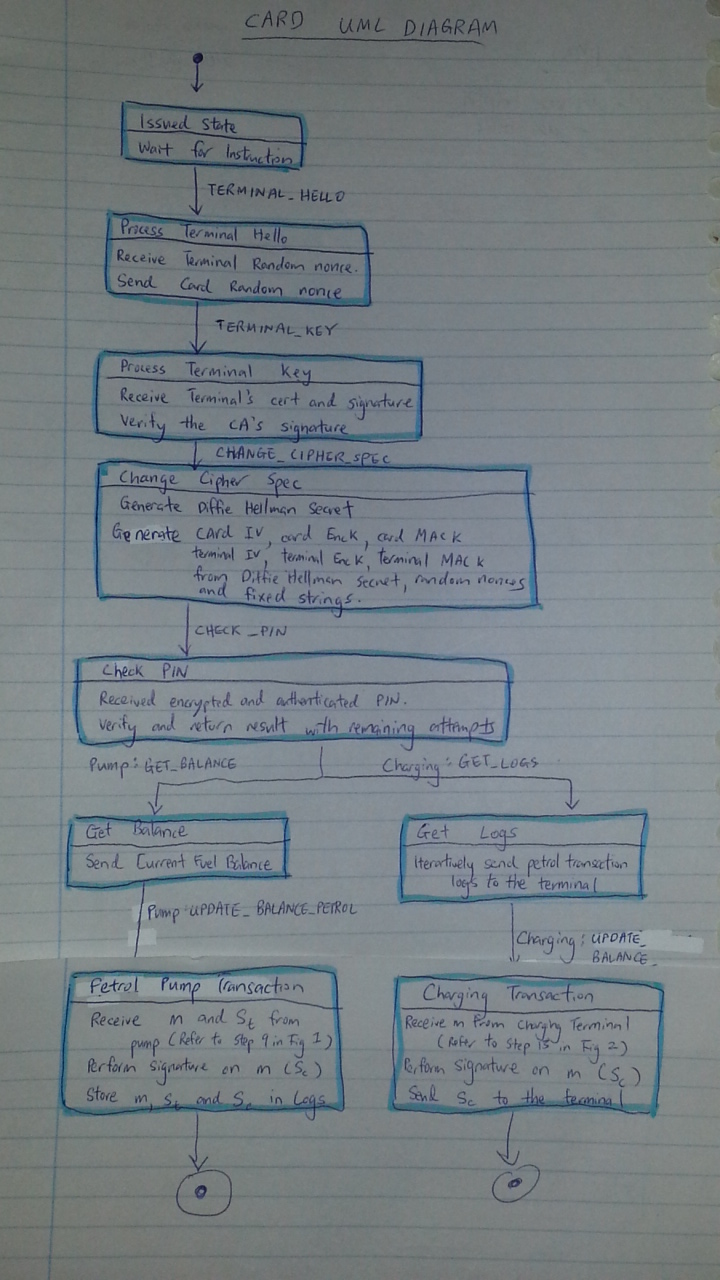
\includegraphics[scale=0.38]{img/state.jpg}
      \caption{\label{figure:state}UML State Diagram. @Saurabh, can you convert this into a nice digital diagram?}
    \end{figure*}



More details of some of the states are provided below:
\subsubsection{Process Terminal Key State}
Mutual Authentication employs ECDH-ECDSA, which employs the SECG curve over a 193 bit binary field. A binary field is chosen to better employ the cryptographic hardware on the smartcard.

\subsubsection{Change Cipher Spec State}
The Card Initialisation Vector (IV) is generated as SHA-1(Terminal Random Nonce, Card Random Nonce, Diffie-Hellman Shared Secret, "Byte representing Card IV"), where the multiple inputs to the SHA-1 are concatenated together. The Card Encryption Key, Card MAC Key, Terminal IV, Terminal Encryption Key and Terminal IV are similarly generated by changing the last input Byte.

\subsubsection{Message Encryption and Authentication in Check PIN State}
AES-128 with PKCS7 padding was chosen for encryption while HMAC with SHA-1 was chosen for message authentication. As padding for AES was not provided by the javacard cryptographic libraries, and we had to manually implement it. Our implementation integrates well with the Terminal's Bouncy castle 'AES-128 with PCKS7' API.

The card sends messages encrypted with the Card Encryption Key, using the card IV as input and authenticated with the Card MAC key. Correspondingly, the terminal sends messages encrypted with the Terminal Encryption Key, using the Terminal IV as input and authenticated with the Terminal MAC key. Card and Terminal can decrypt and verify each other's messages as they have all six keys.

The IVs are updated after each message is sent, using the last sent 16-byte block of that sent message.

\subsubsection{Get Balance, Get Logs, Petrol Pump Transaction and Charging Transaction State}
Transactions with the Petrol and Charging Terminals are implemented very closely to Figure \ref{Design:PetrolPT} and \ref{subsection:chargingterminal} in the design.


\subsection{Database Design}

The designed database consists the backend that stores all the information needed in order to successfully implement the proposed 
protocol. The database was implemented in the beginning without taking into account the limitations that were introduced in 
Chapter \ref{chapter:limitations}. As a result, many of the following details were not implemented in the final application, 
although it was initially desired. This Chapter reports the structure of the database and explains why these choices were made.

To begin with, the table 'card' contains the basic information for every valid card at that moment, Figure \ref{figure:dbtable_card}. 
The ID of the card is the Primary key and BTREE index is used for this attribute. Although the system administrator may search 
for any value, the most common lookup is done by the charging terminal, which searches for the ID of every inserted smart card. Then, 
the terminal (according to \ref{subsection:chargingterminal}) verifies the balance, checks that the card has not been expired, 
checks whether the card has been charged this month, verifies the signature using the public key of the card in the database and, finally, 
updates the necessary fields. All of there attributes are stored in this single table and no other lookup is needed to be 
done by the charging terminal to get the informations of the smart card.
    \begin{figure*}
    	\centering
    	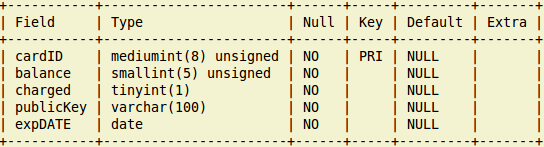
\includegraphics[scale=0.38]{img/dbtable_card.png}
    	\caption{\label{figure:dbtable_card}DB table for all valid cards}
    \end{figure*}
    
Additionally, the table 'log' has an entry for every transaction that has been performed between any smart card and any terminal. In addition to an increasing id that is given to all transactions, the table contains the parts of the message $m$ (common in both protocols \ref{Design:PetrolPT} and \ref{subsection:chargingterminal}) and the signatures of both the involved terminal and the involved smart card. The attributes of the table can be seen in Figure \ref{figure:dbtable_log}. 
    \begin{figure*}
    	\centering
    	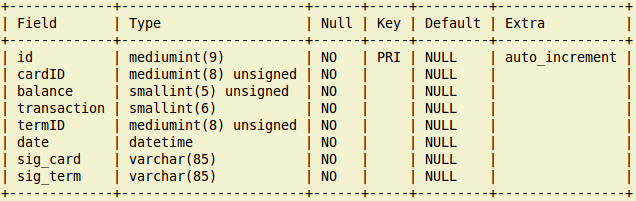
\includegraphics[scale=0.38]{img/dbtable_log.png}
    	\caption{\label{figure:dbtable_log}DB logging table}
    \end{figure*}
    
Finally, there are two extra tables that are not actually used by the application at this moment. Firstly, the table 'terminal' (Figure \ref{figure:dbtable_terminal}) stores the basic informations for every existing terminal and includes a BTREE index for the ID attribute. This attribute, just like the card ID, is supposed to be searched every time that the charging terminal is used. Afterwards, the public key is obtained and used to verify the signature of the terminal. Secondly, the table 'user' stores the basic information for every user of the system. Each row corresponds the user to a card and marks the validity of the card. If the card has changed then the row is marked as invalid and a new entry for the user is entered. As well as the entry of the previous card is removed from the table 'card' and the new one is inserted. The columns can be seen in Figure \ref{figure:dbtable_user}.
    \begin{figure*}
    	\centering
    	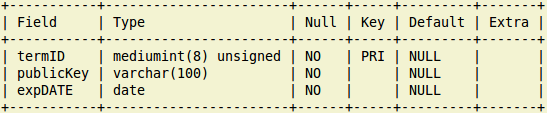
\includegraphics[scale=0.38]{img/dbtable_terminal.png}
    	\caption{\label{figure:dbtable_terminal}DB table for all valid terminals}
    \end{figure*}    
    \begin{figure*}
    	\centering
    	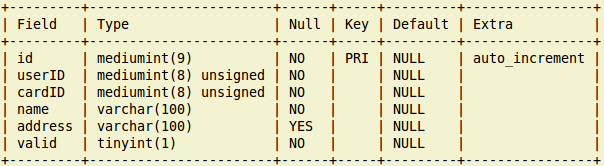
\includegraphics[scale=0.38]{img/dbtable_user.png}
    	\caption{\label{figure:dbtable_user}DB table for every user}
    \end{figure*}
\subsection{Additional protection}

In order to protect transactions between the card and terminals against card tearing, we have implemented atomicity of operations via the JavaCard API. This includes calls to \emph{JCSystem.beginTransaction()}, \emph{JCSystem.commitTransaction()} when the transaction is successful and \emph{JCsystem.abortTransaction()} when the transaction fails because of an internal error or invalid user input (e.g. attempt to pump more petrol than the available balance allows).

Furthermore, the code is modular and designed in such a way that each component returns information regarding the success of an operation. This means that in case of failure, the caller of a method can receive feedback and act according to the success status of an state change.

We also make use of try/catch statements extensively in an attempt to control the execution flow of the program and avoid entirely errors, such that memory corruption. Our team tried to take into consideration both the physical and the software security during the implementation of the petrol rationing system.

\subsection{Notes}
Some interesting observations about javacard APIs and coding environment:

\begin{enumerate}
 \item The cryptographic libraries used by the javacard and terminal are implemented slightly differently. For example, the Diffie-Hellman Key exchange (ALG\_EC\_SVDP\_DH) on Terminal returns a byte array of length 25, while the card returns a byte array of length 20. This is because the Card automatically applies a SHA-1 hash on the EC-point while Terminal does not.
 \item CMAC implementation on the javacard is buggy
\end{enumerate}

\end{document}

